\documentclass[modern]{CORE-AAS/aastex631} 
\usepackage{datetime}
\newcommand{\vdag}{(v)^\dagger}
\newcommand\aastex{AAS\TeX}
\newcommand\latex{La\TeX}
\usepackage{amsmath}
\usepackage{multirow}
\usepackage[abs]{overpic}
\usepackage{breakurl}
\usepackage{hyperref}
\usepackage{textcomp}
\usepackage{fancyhdr}
\usepackage{graphicx}
\usepackage{amssymb}
\usepackage[toc,page]{appendix}
\usepackage{nicefrac}
\usepackage{svg}
\usepackage[utf8]{inputenc}
% Table float box with bottom caption, box width adjusted to content 
\usepackage{varwidth}
\usepackage{scrextend}
\usepackage{xcolor}
\usepackage{colortbl}
\usepackage{tablefootnote}
\usepackage{array}
\usepackage[]{graphicx}
\usepackage{xspace}
%%%%%%%%%%%%%%%%%%%%%%%%%%%%
%%% CAPTION OF FIGURE %%%%%%
%%%%%%%%%%%%%%%%%%%%%%%%%%%%

\newcommand{\SAUNAS}{\texttt{SAUNAS}}
\newcommand{\SAUNA}{\texttt{SAUNA}} %without the last S
\newcommand{\XAUNA}{\texttt{XAUNA}} %testing to see how it looks like 

\newcommand\asr{\ref@jnl{Adv. Space Res.}}%   % Advances in Space Research

\newcommand{\captionOpticalvsChandra}{DSS observations (\emph{left}) vs. \Chandra/ACIS soft band (0.5 -- 1.2 MeV) adaptive smoothed surface brightness maps (\emph{right}, s$^{-1}$ cm$^{-2}$ arcsec $^{-2}$). The white contour in both panels represents the detection limit in soft-band X-ray, defined with as the probability ($p-$value) that the mean flux is compatible with the background ($p_{\rm lim}=0.05$).}

\newcommand{\HI}{\ion{H}{1}}
\newcommand{\et}{et al.}
\newcommand{\kms}{km~s$^{-1}$}
%\newcommand{\s4g}{S$^{4}$G}
\newcommand{\s}{$\sim$}
\newcommand{\n}{$-$}
\newcommand{\Chandra}{\emph{Chandra}}
\newcommand{\Hubble}{\emph{HST}}
\newcommand{\Spitzer}{\emph{Spitzer}}
\newcommand{\Galex}{\emph{GALEX}}
\newcommand{\MASS}{2MASS}
\newcommand{\ciao}{\texttt{CIAO}}
\newcommand{\LIRA}{\texttt{LIRA}}
\newcommand{\vorbin}{\texttt{vorbin}}
\newcommand{\WISE}{\emph{WISE}}
\newcommand{\SDSS}{SDSS}
\newcommand{\CSNG}{\emph{CSNG}}
\newcommand{\GSWLC}{\emph{GSWLC}}
\newcommand{\ud}{\,\mathrm{d}}
\newcommand{\ue}{\,\mathrm{e}}
\newcommand{\mpch}{\,{\it h}^{-1}\, {\rm Mpc}}
\def\square{\vrule height 4.5pt width 4pt depth -0.5pt}
\def\threesquares{\square~\square~\square\ }
\definecolor{navyblue}{rgb}{0.0, 0.0, 0.5}
\def\abremark#1{{\color{navyblue}\threesquares\tt (alex) #1~\threesquares}}
\newcommand{\escmarc}{s$^{-1}$ cm$^{-2}$ arcsec$^{-2}$}
\usepackage{makecell}

\renewcommand\theadalign{bc}
%\renewcommand\theadfont{\bfseries}
\renewcommand\theadgape{\Gape[4pt]}
\renewcommand\cellgape{\Gape[4pt]}


\newcommand{\bxa}{\textt}
\begin{document}
\vspace*{-0.8cm}\noindent{\textcolor{lightgray}{Compiled: \currenttime\ \today\ (UTC)}
\title{SAUNAS II: Discovery of Cross-shaped X-ray Emission and a Rotating Circumnuclear Disk \\in the Supermassive S0 Galaxy NGC 5084}

\begin{abstract}
Combining \Chandra, ALMA, EVLA, and \emph{Hubble} Space Telescope archival data  and newly acquired APO/DIS spectroscopy, we 
detect a double-lobed 17~kpc X-ray emission with plumes oriented approximately perpendicular and parallel to the galactic plane of the massive lenticular galaxy NGC\,5084 at 0.3--2.0~keV. 
We detect a highly inclined ($i=71.2^{+1.8\circ}_{-1.7}$), molecular circumnuclear disk ($D=304^{+10}_{-11}$ pc) in the core of the galaxy rotating (V$^{\rm (2-1) CO}_{\rm rot}=242.7^{+9.6}_{-6.4}$ km s$^{-1}$) in a direction 
perpendicular to that of the galactic disk, implying a total mass of $\log_{10}\left( \frac{M_{\rm BH}}{M_{\odot}} \right) = 7.66^{+0.21}_{-0.15}$ for NGC\,5084's supermassive black hole. Archival EVLA radio observations at 6 cm and 20 cm reveal two symmetric radio lobes aligned with the galactic plane, extending to a distance of $\overline{R}=4.6\pm0.6$ kpc from the core, oriented with the polar axis of the circumnuclear disk. The spectral energy distribution lacks strong emission lines in the optical range. 
Three formation scenarios are considered to explain these multi-wavelength archival observations: 1) AGN re-orientation caused by accretion of surrounding material, 2) AGN-driven hot gas outflow directed along the 
galactic minor axis, or 3) a starburst / supernovae driven outflow at the core of the galaxy. This discovery is enabled by new imaging analysis tools 
including \SAUNAS\ (Selective Amplification of Ultra Noisy Astronomical Signal), demonstrating the abundance of information still to be exploited in the vast and growing astronomical archives.
\end{abstract}

\section{Introduction} \label{sec:intro}
Observational evidence suggests that supermassive black holes (SMBHs; $M_{\rm BH}=10^{6-9.5}$) are present at the core of most massive galaxies \citep{kormendy+2013araa51_511}. The accretion of material by SMBHs has been observed to be tightly connected with the evolution of the entire galaxy, enabling periods of nuclear activity in which the total luminosity of the galaxy is enhanced. 
%"modified" does not imply a direction - the luminosity could increase or decrease. Active Galactic Nuclei \citep[AGNs,][]{mulchaey+1996apj467_197} are powered by the release of gravitational energy in a compact accretion disk surrounding the SMBH at the core of the galaxy, generating emission across the whole electromagnetic spectrum \citep{heckman+2014araa52_589}. 

The main hypothesis of the unified scheme of active galactic nuclei (AGNs) is that the broad range of spectro-photometric properties is caused by the angle of inclination between the observer and an obstructing circumnuclear disk \citep{antonucci1993araa31_473, urry+1995pasp107_803}. The circumnuclear disk is a dusty and molecular gas component of outflowing and inflowing material surrounding the AGN, the so-called `torus'. According to this theory, when AGN's are observed at low inclination angles \citep[$i<45$--$60^{\circ}$, where $i=0^{\circ}$ would be face-on,][]{marin2014mnras441_551}, broad optical and ultraviolet (UV) spectral features (full width at half maximum; FWHM $\geq 1000-20,000$ km s$^{-1}$) are expected, corresponding to the Broad Line Region (BLR); a bright, non-stellar, central compact source visible at all wave-lengths, and with low polarization degree \citep[Type 1 AGNs,][]{netzer2015araa53_365}. At higher inclination angles, the BLR would be obscured by the torus showing only the narrow line region emission (NLR, Type 2 AGNs). See \citet{peterson2006incollection_77, netzer2015araa53_365, ramosalmeida+2017nat1_679} for reviews in the field.

A large fraction of the total mass of SMBHs is thought to have been accreted during the peak of quasar activity in the early Universe \citep[$z=2-3$,][]{boyle+1998mnras293_49, delvecchio+2014mnras439_2736, madau+2014araa52_415}. During that period ($z\sim2-3$), the star-formation rate (SFR) and SMBH growth rate peaked and then decreased by a factor of ten from $z=1$ to the local Universe \citep{shankar+2009apj690_20}. The observed decrease in SFR is coincident with one of the most notable changes in the population of galaxies: the decline of the population of spirals and the rise of lenticular galaxies in the Local Universe \citep{dressler+1997apj490_577}.

\begin{figure*}[t!]
\begin{center}
 % trim left bottom right top 
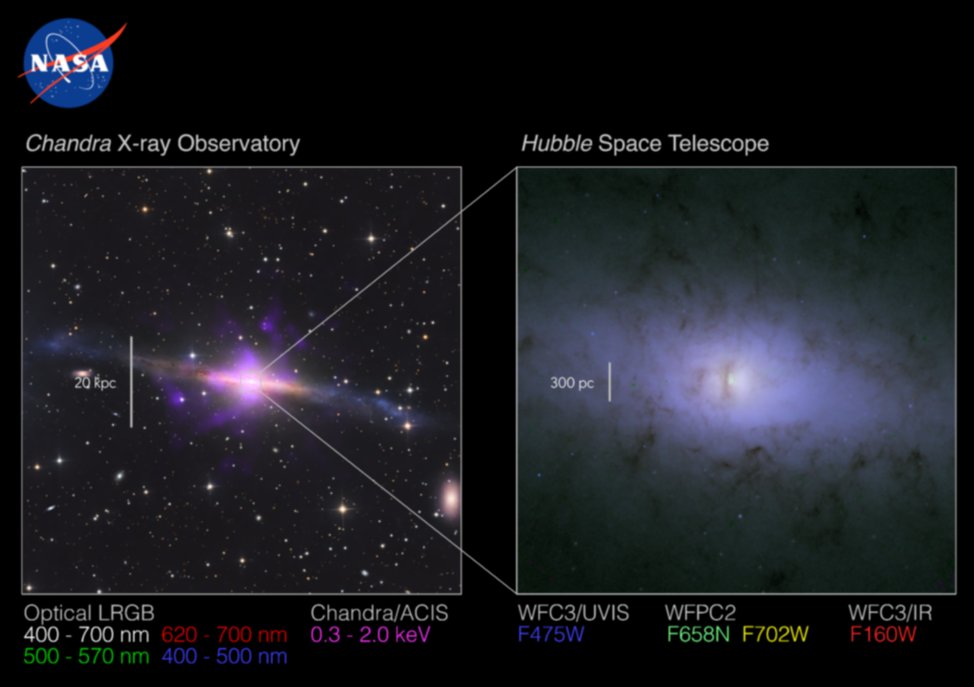
\includegraphics[trim={0 10 0 100}, clip, width=\textwidth]{FIGURES/Composition_NGC5084_poster_v6_paper.png}
\caption{Morphological structure of NGC\,5084 in X-ray, optical, and near-infrared wavelengths. \emph{Left panel:} Optical and X-ray image of 
the disk of NGC\,5084. \emph{Background:} Luminance-RGB image (Telescope: CDK17. Camera: SBIG STXL-11002M. Filter: Astrodon Gen 1 LRGB E-Series. Credit: Martin Pugh \& Brian Diaz). Field-of-view (FOV): $15\times15$ arcmin$^{2}$. \emph{Right panel:} High resolution luminance-RGB image zoom of the core of NGC\,5084 based on \emph{Hubble} Space Telescope observations. \emph{Blue:} WFC3/UVIS F475W. \emph{Green:} WFPC2 F658N. \emph{Yellow:} WFPC2 F702W. \emph{Red:} WFC3/IR F160W.  FOV: $24\times24$ arcsec$^{2}$. See the legend for color-band description and the physical scale-bars in the panels for reference.} 
\label{fig:NGC5084_poster}
\end{center}
\end{figure*}

\subsection{Chandra X-ray Observatory} \label{sec:data_chandra}

\Chandra/ACIS is particularly well-suited to detect hot gas emission in galaxies, due to its high-sensitivity in the 0.3-2.0 keV range and the high spatial resolution that allows masking of contamination from point sources. \Chandra/ACIS observations are reduced following the \SAUNAS\ pipeline, a methodology presented in \texttt{SAUNAS I}, which specializes in the detection of low surface brightness emission from \Chandra/ACIS observations. \SAUNAS\ comprises several steps for calibration including: 1) standard pre-calibration using \texttt{CIAO}, 2) automatic point spread function modeling and deconvolution, 3) estimation of the uncertainties via bootstrapping and Monte Carlo simulations, and 4) adaptive Voronoi binning. \par 
The two main products of \SAUNAS\ are surface brightness and signal-to-noise ratio maps, allowing the observer to identify potential sources and their extension up to a certain statistical limit. Since the objective is to identify the underlying shape of the X-ray extended emission in NGC\,5084, PSF deconvolution is a particularly critical step. \citet{borlaff+2024apj967_169} provides a full description of the methodology.

\subsection{Hubble Space Telescope Imaging} \label{sec:data_hst}

\emph{Hubble} Space Telescope observations of NGC\,5084 are available at the Mikulski Archive for Space Telescopes\footnote{\url{https://mast.stsci.edu/portal/Mashup/Clients/Mast/Portal.html}} (MAST, \dataset[doi: 10.17909/j04e-sq50]{https://doi.org/10.17909/j04e-sq50}). In particular, we focus on high-resolution imaging observations obtained with WFPC2 (Proposal PI: Malkan, Matthew A.,
Proposal ID: 6785, F702W and F658N, June 1996), WFC3/IR (F160W, Proposal PI: Boizelle, Benjamin, Proposal ID: 15909, and WFC3/UVIS (F475W, same Proposal ID as WFC3/IR, see Table \ref{tab:Observations}). Planetary Camera (PC) observations of WFPC2 allow for an angular resolution of $0.05$ arcsec, while WFC3s IR and UVIS channels have a resolution of $0.13$ and $0.04$ arcsec respectively. At a distance of $D=	29.91\pm2.12$~Mpc \citep[6.90~arcsec~kpc$^{-1}$,][]{koribalski+2004aj128_16}, and assuming a Nyquist sampled PSF, the physical spatial resolution scales are $\sim12$ pc (WFC3/UVIS) and $\sim36$ pc (WFC3/IR), respectively. Table\,\ref{tab:Observations} summarizes the available observations.

\cite{pan+2019apj881_119}
\ref{fig:NGC5084} in section \ref{subsec:results_xray_ima}
\subsection{Optical spectroscopic observations} \label{subsec:data_optical_spectra}

\section{Results} \label{sec:results}

Figure \,\ref{fig:NGC5084} presents the new \SAUNAS-processed images in the selected broad X-ray band (0.3--2.0 keV), overlayed on the optical morphology of the galaxy \citep[large FOV optical and near-infrared $gri$ image from Pan-STARRS, ][]{chambers+2016arXiv1612.05560}. Additionally, Fig.\,\ref{fig:NGC5084_per_band} in Appendix \ref{Appendix:Xray_subbands} shows the three X-ray (\emph{soft:} 0.3-1.0 keV, \emph{medium:} 1.0-2.0 keV, \emph{hard:} 2.0 - 8.0 keV) bands. \par 

In order to verify the results from the pipeline, we study the significance of the extended emission in Appendix \ref{Appendix:Xray_noPSFdeco_test} using two different, additional methodologies widely used in the literature. First, we determine if there is an excess of emission around the bright core of the galaxy by comparing the PSF surface brightness profile with the observed profile in the original \Chandra/ACIS observations, without applying Voronoi binning or PSF deconvolution. This methodology has been extensively used in the literature \citep{fabbiano+2017apj842_4,fabbiano+2018apj855_131, jones+2020apj891_133,ma+2020apj900_164,ma+2023apj948_61} to identify hot gas halos and other extended emission components. The results (see Fig.\,\ref{fig:NGC5084_psf_profile}) show a clear excess of emission above that expected PSF scattering up to the same radial distance as predicted by the $3\sigma$ contours on Fig.\,\ref{fig:NGC5084}, confirming that the X-ray emission of NGC\,5084 is not caused by PSF-scattered light from the bright core and that the extended emission is significant.

\bibliography{Extragalactic}\bibliographystyle{CORE-AAS/aasjournal}

\end{document}

